\documentclass[11pt,a4paper]{article}

\usepackage[margin=2.5cm]{geometry}
\usepackage{graphicx}
\usepackage{booktabs}
\usepackage{longtable}
\usepackage{amsmath}
\usepackage{xcolor}
\usepackage{hyperref}
\usepackage{fancyhdr}
\usepackage{caption}
\usepackage{subcaption}
\usepackage{enumitem}
\usepackage{tikz}
\usetikzlibrary{shapes.geometric,arrows.meta,positioning,calc}

\hypersetup{
  colorlinks=true,
  linkcolor=blue!50!black,
  citecolor=blue!50!black,
  urlcolor=blue!50!black
}

\pagestyle{fancy}
\fancyhf{}
\fancyhead[L]{EMINES UM6P -- UFAM Research Internship}
\fancyhead[R]{Garimpo Detection from Satellite Imagery}
\fancyfoot[C]{\thepage}
\renewcommand{\headrulewidth}{0.4pt}

\title{\textbf{Automated Detection of Illegal Gold-Mining\\
Barges (Garimpo) on the Rio Madeira Using Optical\\
Satellite Imagery}\\[0.3cm]
\large Progress Report II --- Research Internship}

\author{
ABDELOUALI Rachid \quad EL HAMDAOUI Fares \quad ECH-CHAFIY Soufiane\\[0.15cm]
\small EMINES School of Industrial Management, Universit\'e Mohammed VI Polytechnique (UM6P)\\[0.3cm]
\normalsize In collaboration with\\
\small Universidade Federal do Amazonas (UFAM)\\[0.3cm]
\small Supervisor(s): Naziano Filizola
}

\date{August 22, 2026}

\begin{document}

\maketitle

\begin{abstract}
This report documents the second stage of a joint EMINES UM6P--UFAM research
internship building an automated, learning-based detector for garimpo (illegal
gold-mining) activity on the m\'edio Rio Madeira from CBERS 4A optical imagery,
extending the manual-digitizing methodology of Monteiro (2024) and the
first-stage pipeline reported previously. Since the previous report, the dataset
has been re-audited and corrected (1,292 usable tiles, 38 positive / 1,254
negative, following the removal of one label found to sit on a mosaic-seam
artifact), a supervised segmentation model has been designed, trained, and
evaluated (a pretrained ResNet18 U-Net predicting a per-pixel garimpo
probability heatmap), and a full-scene sliding-window inference pipeline has
been built and validated: on the held-out validation footprint, every one of
five known garimpo sites is recovered with near-maximal confidence and no
false positives elsewhere in the scene, while a scan of a scene with zero
labeled sites surfaces a small number of candidate false positives, most of
which trace to a documented image-artifact sensitivity and a minority of which
remain genuinely ambiguous. Aggregated across all 13 available scenes, the
detector achieves 100\% recall and 30.4\% raw precision (43.6\% once
artifact-linked false positives are excluded) at a probability threshold of
0.5. A first prototype interactive map interface has also been built,
overlaying model output on a real satellite basemap using footprint
coordinates recovered from CBERS product metadata. This report details the
methodology, the diagnostic process behind each of these results, and the
concrete next steps required before the pipeline can be considered a reliable
detection tool.
\end{abstract}

\section{Introduction}

Gold mining along the Rio Madeira has been an active, continuous practice
since at least the early 1980s, evolving from small manual operations on the
riverbanks into a mechanized industry built around suction dredges mounted on
floating barges (Bastos and Lacerda, 2004). Because extraction takes place
underwater, this activity leaves almost none of the surface signatures
typically associated with terrestrial mining (e.g. exposed pits, tailings
piles), which makes remote detection considerably harder than for land-based
illegal mining. The barges and dredges themselves --- along with the sediment
plumes, sandbanks and bar deposits they leave behind --- are in practice the
only reliably observable indicators of the activity from space.

This project is carried out as part of a research internship agreement
between the EMINES School of Industrial Management (UM6P), Morocco, and the
Departamento de Geoci\^encias (DEGEO), Universidade Federal do Amazonas
(UFAM), Brazil. It builds directly on the undergraduate thesis of Anna
Beatriz de Oliveira Monteiro (Monteiro, 2024), which established the manual
methodology and generated four years (2020--2023) of visually-digitized barge
locations along a stretch of the m\'edio Rio Madeira. This report covers the
CBERS 4A optical detection track specifically; a parallel Sentinel-1/Sentinel-2
fusion track, developed by other members of the internship team, is reported
separately.

\subsection{Objectives}
\begin{itemize}[nosep]
  \item Build a reproducible image-processing pipeline that isolates the
        river channel and produces analysis-ready tiles from raw CBERS 4A
        scenes.
  \item Construct a labeled image dataset (garimpo present / absent, with
        bounding boxes) from the available batch of CBERS 4A scenes, and
        audit it for data-quality issues before training.
  \item Train and evaluate a small-data-appropriate segmentation model that
        outputs a per-pixel garimpo probability heatmap, rather than a
        classification label alone.
  \item Extend detection from individual tiles to full, arbitrarily large
        scenes via sliding-window inference, and quantify precision/recall
        across the full available dataset.
  \item Build a first prototype for visualizing detector output on a real
        geographic map, as a step toward a deployable monitoring tool.
\end{itemize}

\section{Study Area and River Characteristics}

The study area is located on the m\'edio Rio Madeira, in the municipality of
Manicor\'e, Amazonas State, Brazil, within the same reach studied by Monteiro
(2024). Table~\ref{tab:river} summarizes the key physical characteristics of
the Rio Madeira basin relevant to this work.

\begin{table}[htbp]
\centering
\caption{Key physical characteristics of the Rio Madeira basin.}
\label{tab:river}
\begin{tabular}{ll}
\toprule
\textbf{Characteristic} & \textbf{Value / Description} \\
\midrule
Drainage basin area & $\sim$1,324,727 km$^2$ (largest Amazon sub-basin) \\
Share of Amazon basin & $\sim$23\% \\
Mean annual discharge & $\sim$26,500 m$^3$/s \\
Origin & Andes Cordillera (Beni, Madre de Dios, Mamor\'e rivers) \\
Hydrological regime & Tropical austral (single annual flood peak, $\sim$April; \\
                     & low water $\sim$September--October) \\
Channel pattern & Anabranching, locally straight to meandering; straight \\
                & reaches up to $\sim$35 km \\
Water characteristics & pH 6.5--7, high electrical conductivity, high \\
                       & suspended sediment load \\
Gold transport mechanism & Secondary (alluvial) gold, transported as \\
                          & bedload/suspended sediment from Andean source rocks \\
\bottomrule
\end{tabular}
\end{table}

The strong seasonal (vazante/enchente) cycle is particularly relevant to this
project: barge activity is known to be inversely related to water level, with
more barges operating during low water (roughly July--December) than during
the flood peak (Monteiro, 2024).

\section{Prior Work: Monteiro (2024)}

The foundation for this project is the undergraduate thesis of Monteiro
(2024), developed at UFAM under the supervision of Prof.\ Naziano Pantoja
Filizola J\'unior. Her work is, to our knowledge, the first systematic
attempt to identify and quantify garimpo barges on the m\'edio Rio Madeira
using a combination of optical (CBERS 4A) and radar (Sentinel-1A) imagery.

\subsection{Methodology summary}
Monteiro processed CBERS 4A WPM imagery in QGIS (RGBN band composition
followed by pansharpening with the 2 m panchromatic band), and processed
Sentinel-1A dual-polarization (VV/VH) imagery in SNAP, generating three
derived RGB products (Dual Pol Ratio, Dual Pol Difference, Dual Pol
Multiple). Barges and dredges were then identified and digitized manually,
as point vector features, directly in QGIS --- no automated or
learning-based detection was used at any stage.

\subsection{Key findings}
\begin{itemize}[nosep]
  \item CBERS 4A optical imagery, at 2 m pansharpened resolution, allowed
        clear visual identification and counting of barges, though it could
        not distinguish barges from dredges specifically.
  \item Sentinel-1 SAR was able to detect some metallic-hulled vessels as
        bright backscatter points even under cloud cover, but detected far
        fewer vessels overall than the optical imagery in the available
        image dates.
  \item Barge counts varied strongly by season and year, ranging from as few
        as 24 (June 2021) to as many as 241 (June 2020) across the study
        reach.
  \item Barge locations correlated spatially with fluvial bars and alluvial
        deposits, consistent with the known alluvial origin of Madeira River
        gold.
\end{itemize}

\section{Remote Sensing Background}

\subsection{How satellite remote sensing informs this problem}
Every satellite sensor used in this project trades off three resolutions:
spatial resolution, spectral resolution, and temporal resolution. Detecting a
garimpo barge --- an object typically only a few meters to a few tens of
meters long --- is fundamentally a spatial-resolution problem: it requires
imagery fine enough to resolve a small target against a highly textured water
background.

\subsection{Why CBERS 4A at 2 m resolution}
CBERS 4A WPM pansharpened imagery (2 m spatial resolution) was selected as
the primary data source for this project for three reasons: (1) resolution
adequacy --- a barge on the order of 10--20 m in length spans roughly 5--10
pixels; (2) continuity with prior work --- using the same sensor as Monteiro
(2024) allows direct comparison on overlapping dates; (3) cost and access ---
CBERS 4A imagery is freely distributed by INPE.

\section{Data and Methodology}

Figure~\ref{fig:pipeline} gives an overview of the full processing pipeline
described in this section and Sections~\ref{sec:audit}--\ref{sec:geomorph},
from raw scene acquisition through full-scene detection and false-positive
root-cause analysis.

\begin{figure}[htbp]
\centering
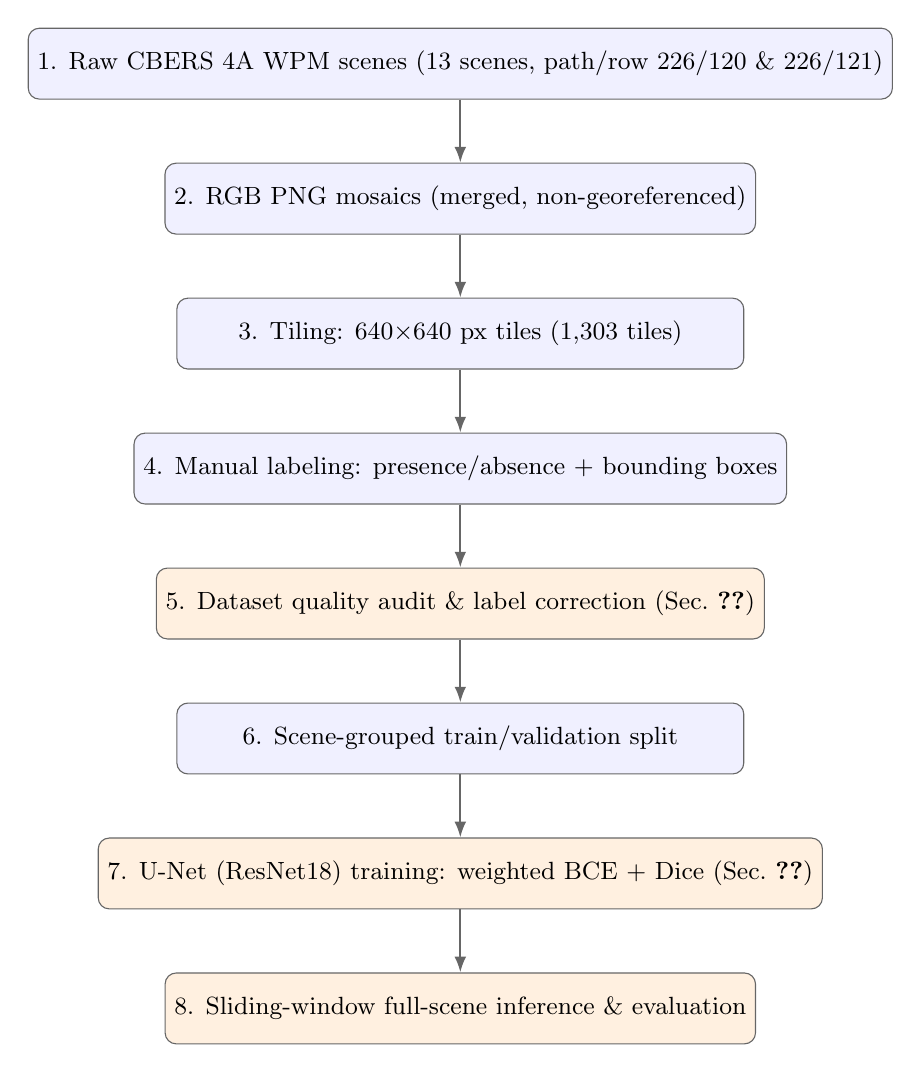
\begin{tikzpicture}[
  node distance=8mm,
  box/.style={rectangle, rounded corners, draw=black!60, fill=blue!6,
              minimum width=7.2cm, minimum height=9mm, align=center,
              font=\small},
  boxnew/.style={rectangle, rounded corners, draw=black!60, fill=orange!12,
              minimum width=7.2cm, minimum height=9mm, align=center,
              font=\small},
  arr/.style={-{Latex[length=2mm]}, thick, black!60}
]
\node[box] (n1) {1. Raw CBERS 4A WPM scenes (13 scenes, path/row 226/120 \& 226/121)};
\node[box, below=of n1] (n2) {2. RGB PNG mosaics (merged, non-georeferenced)};
\node[box, below=of n2] (n3) {3. Tiling: 640$\times$640 px tiles (1,303 tiles)};
\node[box, below=of n3] (n4) {4. Manual labeling: presence/absence + bounding boxes};
\node[boxnew, below=of n4] (n5) {5. Dataset quality audit \& label correction (Sec.~\ref{sec:audit})};
\node[box, below=of n5] (n6) {6. Scene-grouped train/validation split};
\node[boxnew, below=of n6] (n7) {7. U-Net (ResNet18) training: weighted BCE + Dice (Sec.~\ref{sec:model})};
\node[boxnew, below=of n7] (n8) {8. Sliding-window full-scene inference \& evaluation};
\foreach \a/\b in {n1/n2,n2/n3,n3/n4,n4/n5,n5/n6,n6/n7,n7/n8}
  \draw[arr] (\a) -- (\b);
\end{tikzpicture}
\caption{Overview of the full processing pipeline. Orange stages (5, 7--8)
are new since the previous report.}
\label{fig:pipeline}
\end{figure}

\subsection{Data acquisition and format}
Twelve CBERS 4A WPM scenes were originally acquired covering path/row 226/120
and 226/121 across multiple acquisition dates between 2020 and 2023.
A subsequent, more detailed count of the raw scenes revealed a thirteenth
scene, 2021-10-15 (226/121), which contains zero labeled positive tiles and
had therefore not been separately counted in the earlier scene inventory; it
is included in the present analysis as a genuine true-negative scene and
proves useful as a specific diagnostic case later in this report
(Section~\ref{sec:falsepos}).

During pipeline development, the original raw 4-band GeoTIFFs became
unavailable locally (only RGB-merged, non-georeferenced PNG mosaics remained
from an earlier processing pass). A deliberate scope decision was made to
proceed with model development on this RGB PNG data --- without the near-infrared
band and without native georeferencing --- rather than lose development
time re-acquiring the raw imagery. This is documented explicitly because it
shapes several downstream design choices (Section~\ref{sec:model}) and is
revisited as a concrete next step (Section~\ref{sec:nextsteps}). The original
georeferenced 4-band TIFF products (BAND0--BAND4, with accompanying XML
metadata) were subsequently located in a project data mirror and used later
in this report specifically to recover approximate scene footprint
coordinates as groundwork for a planned interactive map interface (see
Section~\ref{sec:nextsteps}); they have not yet been reintroduced into the
model training pipeline itself.
Figure~\ref{fig:rawscene} shows a representative full raw scene.

\begin{figure}[htbp]
\centering
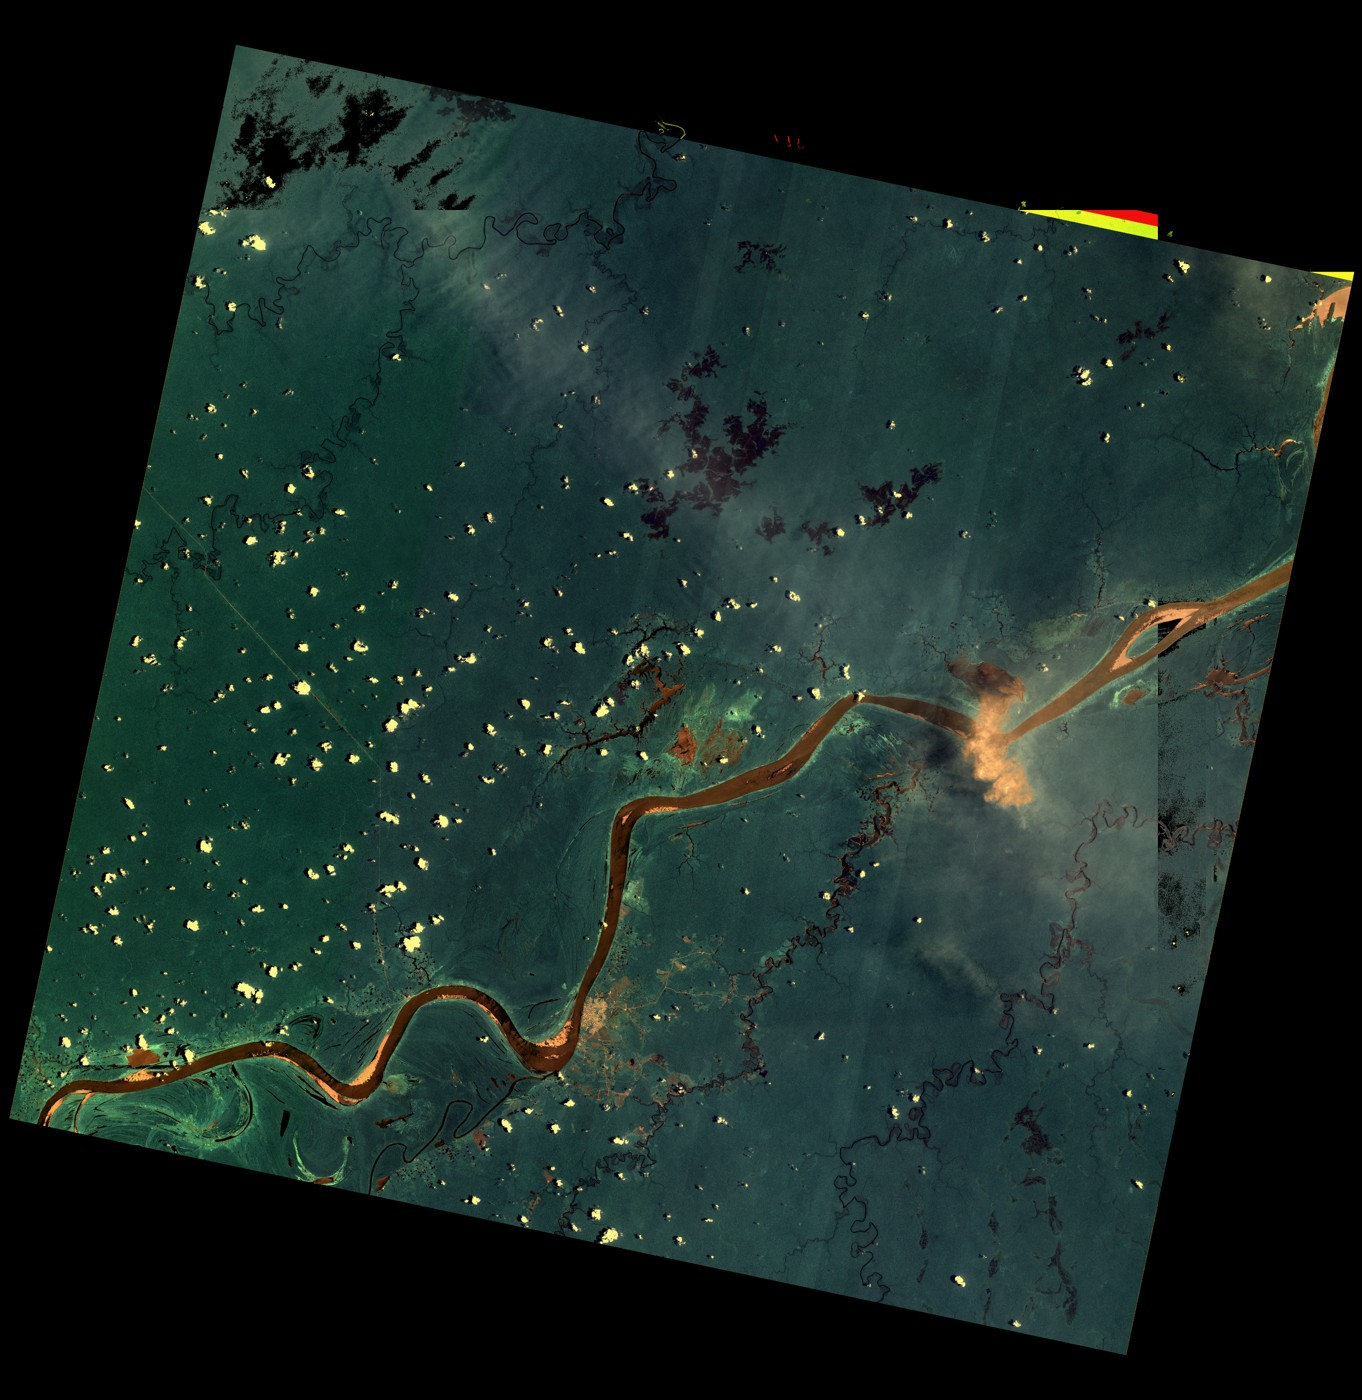
\includegraphics[width=0.75\textwidth]{figures/fig_raw_scene.jpg}
\caption{Representative full CBERS 4A WPM scene (15 October 2021, path/row
226/120), as merged to RGB PNG. The rotated diamond-shaped content region
against black padding reflects the sensor's actual (non north-aligned)
scan geometry within a north-up padded export canvas, confirmed against
CBERS product metadata.}
\label{fig:rawscene}
\end{figure}

\subsection{Tiling}
Each of the merged RGB PNG mosaics was divided into fixed $640 \times 640$
pixel tiles. This produced 1,303 tiles in total across the 13 scenes.

\subsection{Labeling scheme}
Tiles are labeled with a three-way scheme: \textit{positive} (at least one
garimpo barge/dredge visually identifiable), \textit{negative} (no barge
visible), or \textit{uncertain} (pending review, excluded from training and
evaluation). Positive tiles are additionally annotated with pixel-space
bounding boxes around each visible barge/dredge.

\section{Labeling Results}

Manual labeling was completed for all 1,303 tiles. Table~\ref{tab:labels}
gives the final counts, following a data-quality audit and one label
correction detailed in Section~\ref{sec:audit}.

\begin{table}[htbp]
\centering
\caption{Final labeling results, post-audit.}
\label{tab:labels}
\begin{tabular}{lr}
\toprule
\textbf{Category} & \textbf{Count} \\
\midrule
Tiles generated & 1,303 \\
Uncertain (excluded from training/evaluation) & 11 \\
Usable tiles (positive + negative) & 1,292 \\
Negative & 1,254 \\
Positive & 38 \\
Bounding boxes drawn (positive tiles) & 42 \\
\bottomrule
\end{tabular}
\end{table}

The overall positive rate is low ($\sim$2.9\% of usable tiles), consistent
with the sparse, mobile nature of garimpo barges relative to the total
river-corridor area covered. At the pixel level the imbalance is far more
extreme: across the training split alone, positive pixels make up
approximately 0.0025\% of all pixels (a raw negative:positive pixel ratio of
roughly 40{,}000:1), which directly shapes the loss design in
Section~\ref{sec:model}.

\section{Dataset Quality Audit}
\label{sec:audit}

Before committing to a training run, the labeled dataset was audited for a
specific, plausible failure mode: garimpo boxes located near mosaic seams or
sensor nodata regions, which could let a model learn to associate the
\emph{artifact} rather than the actual garimpo signature with a positive
label.

\subsection{Methodology}
For every positive-tile bounding box, the nearest sufficiently large
($>$500 px) near-black connected region in the same tile was located, and the
pixel distance from the box to that region was computed. Boxes within 100 px
of such a region were flagged for manual visual review. Flagged blobs were
further split into two categories: those touching the tile's outer border
(consistent with a genuine mosaic/nodata seam) and those fully interior to
the tile (more consistent with an ordinary cloud shadow, which is common,
benign image content rather than a data defect).

\subsection{Findings}
An initial pass flagged 10 of 43 boxes (across 39 positive tiles) within the
100 px threshold; 7 of these touched a tile border and 3 were interior.
Manual visual inspection of all 7 border-touching cases confirmed a real
mosaic-seam or nodata artifact adjacent to the labeled box in each case, with
one case in particular --- a box only 1.41 px from the seam boundary, visibly
on the dark side of a hard stitching line --- judged unambiguous enough to
warrant exclusion. The remaining 6 border-touching cases, and the 3 interior
(cloud-shadow-adjacent) cases, were kept: a plausible, if not provable,
explanation exists for each (garimpo sites plausibly cluster near
river-adjacent scene boundaries for genuine geographic reasons; cloud shadows
are ordinary scene content), and removing labels on a hunch would trade one
bias for another.

The one clearly contaminated label (tile
\texttt{..\_20230728\_226\_120\_..\_x512\_y4096.png}, box coordinates
$(270, 477)$--$(292, 512)$) was reclassified from positive to negative, its
box removed, and its rasterized mask regenerated as all-zero. A repeat of the
audit on the corrected dataset confirms the fix: 9 of 42 remaining boxes
flagged, 6 border-touching, 3 interior --- exactly one fewer than before, and
no other counts perturbed. This finding, and the full per-box distance table,
is documented in \texttt{docs/dataset\_limitations.md} in the project
repository for methodological transparency.

\section{Deep Learning Detector}
\label{sec:model}

\subsection{Architecture and loss design}
A U-Net-style segmentation model was chosen over a bounding-box object
detector, since the pixel-space bounding-box labels can be rasterized
directly into training masks (filled rectangles) and the resulting model
output --- a per-pixel probability map --- matches the desired final
deliverable (a continuous garimpo-probability heatmap) without any
post-processing conversion step.

The encoder is a ResNet18 backbone pretrained on ImageNet, fully fine-tuned
(not frozen), with a 3-channel RGB input (matching the available data;
Section~\ref{sec:nextsteps} discusses reintroducing the near-infrared band).
A pretrained encoder was preferred over training from scratch given the
limited data budget (1,002 training tiles, 30 positive): low- and mid-level
convolutional filters learned on natural images transfer usefully even under
the domain shift to satellite RGB imagery, and a from-scratch encoder would
spend much of its limited data budget relearning generic filters. ResNet18
specifically (rather than a deeper ResNet34/50) was chosen to limit
overfitting risk given how few positive examples are available.

The loss function combines weighted binary cross-entropy and Dice loss in
equal proportion. Given the extreme pixel-level class imbalance
(Section~\ref{sec:audit}), a positive-class weight for the BCE term is
computed directly from training-set pixel statistics each run, then capped
at 50 to prevent gradient instability from the raw $\sim$40{,}000:1 ratio;
Dice loss, being scale-invariant to class frequency, does most of the
imbalance-handling work. All three loss components (BCE, Dice, and the
combined objective) are logged separately per epoch for diagnosis.

Formally, let $z_i$ denote the model's raw output (logit) at pixel $i$,
$p_i = \sigma(z_i) = 1/(1+e^{-z_i})$ the predicted probability after the
sigmoid, and $y_i \in \{0,1\}$ the ground-truth label at that pixel, over
the $N$ pixels of a tile. The weighted binary cross-entropy is

\begin{equation}
\mathrm{BCE} = -\frac{1}{N} \sum_{i=1}^{N} \Big[ w_{\mathrm{pos}} \, y_i \log(p_i) \;+\; (1-y_i)\log(1-p_i) \Big],
\label{eq:bce}
\end{equation}

which is simply the average, per-pixel penalty for how wrong and how
confident each individual prediction was, with positive-class pixels
counted $w_{\mathrm{pos}}$ times more heavily than negative ones. The
weight itself is computed from the training split each run rather than
fixed by hand,

\begin{equation}
w_{\mathrm{pos}} = \min\!\left( \frac{N_{\mathrm{neg}}}{N_{\mathrm{pos}}},\; 50 \right),
\label{eq:posweight}
\end{equation}

where $N_{\mathrm{neg}}$ and $N_{\mathrm{pos}}$ are the total negative and
positive pixel counts across the training masks; the uncapped ratio is
approximately 40{,}000:1 (Section~\ref{sec:audit}), so the cap at 50 is
strongly binding in practice --- without it, the rare positive pixels would
dominate the gradient by a factor large enough to destabilize training.

The Dice coefficient, by contrast, does not treat pixels independently; it
measures the overlap between the predicted and true positive regions as a
whole,

\begin{equation}
\mathrm{Dice} = \frac{2\sum_{i=1}^{N} p_i y_i + \epsilon}{\sum_{i=1}^{N} p_i + \sum_{i=1}^{N} y_i + \epsilon}, \qquad
\mathcal{L}_{\mathrm{Dice}} = 1 - \mathrm{Dice},
\label{eq:dice}
\end{equation}

with a small smoothing constant $\epsilon$ added to both numerator and
denominator to keep the loss well-defined on all-negative tiles (where
$\sum y_i = 0$). Unlike BCE, Dice is computed entirely from the positive
pixels and their overlap --- the vast negative background contributes
nothing to it once the model is confidently predicting near-zero there, so
it does not benefit from the same easy, aggregate improvement that drives
BCE down quickly in early training (Section~\ref{sec:model}, and
Figure~\ref{fig:lossdecomp} below). The two are combined in equal
proportion,

\begin{equation}
\mathcal{L} = \lambda_{\mathrm{BCE}} \cdot \mathrm{BCE} + \lambda_{\mathrm{Dice}} \cdot \mathcal{L}_{\mathrm{Dice}}, \qquad
\lambda_{\mathrm{BCE}} = \lambda_{\mathrm{Dice}} = 0.5,
\label{eq:combined}
\end{equation}

and it is exactly this combination --- an average over $N$ pixels
dominated numerically by easy negatives (Eq.~\ref{eq:bce}) alongside a
term that only ever looks at the sparse positive region
(Eq.~\ref{eq:dice}) --- that produces the checkpoint-selection behavior
documented in Section~\ref{sec:model}: the two terms are not measuring the
same thing, and do not necessarily reach their best value at the same
training epoch.

Conservative, geospatially-appropriate data augmentation is applied during
training only: horizontal/vertical flips, 90\textdegree{} rotations, and
small brightness/contrast jitter, with spatial transforms applied jointly to
image and mask and photometric transforms applied to the image only.
A weighted sampler oversamples positive tiles during training, since plain
random shuffling at batch size 8 would yield an expected 0.25 positive tiles
per batch given the base class distribution.

\subsection{Training infrastructure and data split}
Initial CPU benchmarking (single forward/backward pass, 640$\times$640
input) measured approximately 1 second per sample, projecting to roughly 6--8
hours for a full 20-epoch training run --- impractical for iterative
development. Training was therefore moved to a GPU-backed environment
(Google Colab, free tier), reducing full 20-epoch runs to approximately
40--45 minutes each.

The dataset was split at the \emph{scene} level, not the tile level, to
avoid leakage between spatially or temporally adjacent tiles. Given only 38
positive tiles spread across 13 scenes, an exhaustive search over all
scene subsets (computationally trivial at this scale) was used to find the
train/validation partition minimizing combined deviation from a target
80/20 split, on both tile-count and positive-count fraction, while
rejecting any candidate with zero positive tiles in validation. This
produced a 10-scene training split (1,002 tiles, 30 positive) and a 3-scene
validation split (290 tiles, 8 positive).

A specific limitation was identified and documented: the dataset spans only
two distinct geographic footprints (path/row 226/120 and 226/121), each
reimaged at roughly six different dates. No scene-level split --- however
well balanced --- can therefore be fully independent in the geographic
sense; the same river bends and mining sites can appear in both the training
and validation splits at different dates. A fully footprint-independent
split exists (all of one footprint in validation) but would push the
validation fraction to 38.5\% of all tiles, an unacceptable reduction in
training data given how few positive examples exist. Given this constraint,
and given that a genuinely independent held-out test set would inherit the
same limitation, a three-way train/validation/test split was deliberately
not pursued; validation performance is reported as a development signal
useful for model selection and gross-overfitting detection, understood to
be a measure of generalization across imaging \emph{dates} at fixed
locations rather than to genuinely new locations.

\subsection{Training results and checkpoint selection}
Three full training runs were performed (20 epochs each, fixed seed),
the first two using the pre-audit labels and the third using the corrected
labels from Section~\ref{sec:audit}. Figure~\ref{fig:training} shows the
final run's training curves.

\begin{figure}[htbp]
\centering
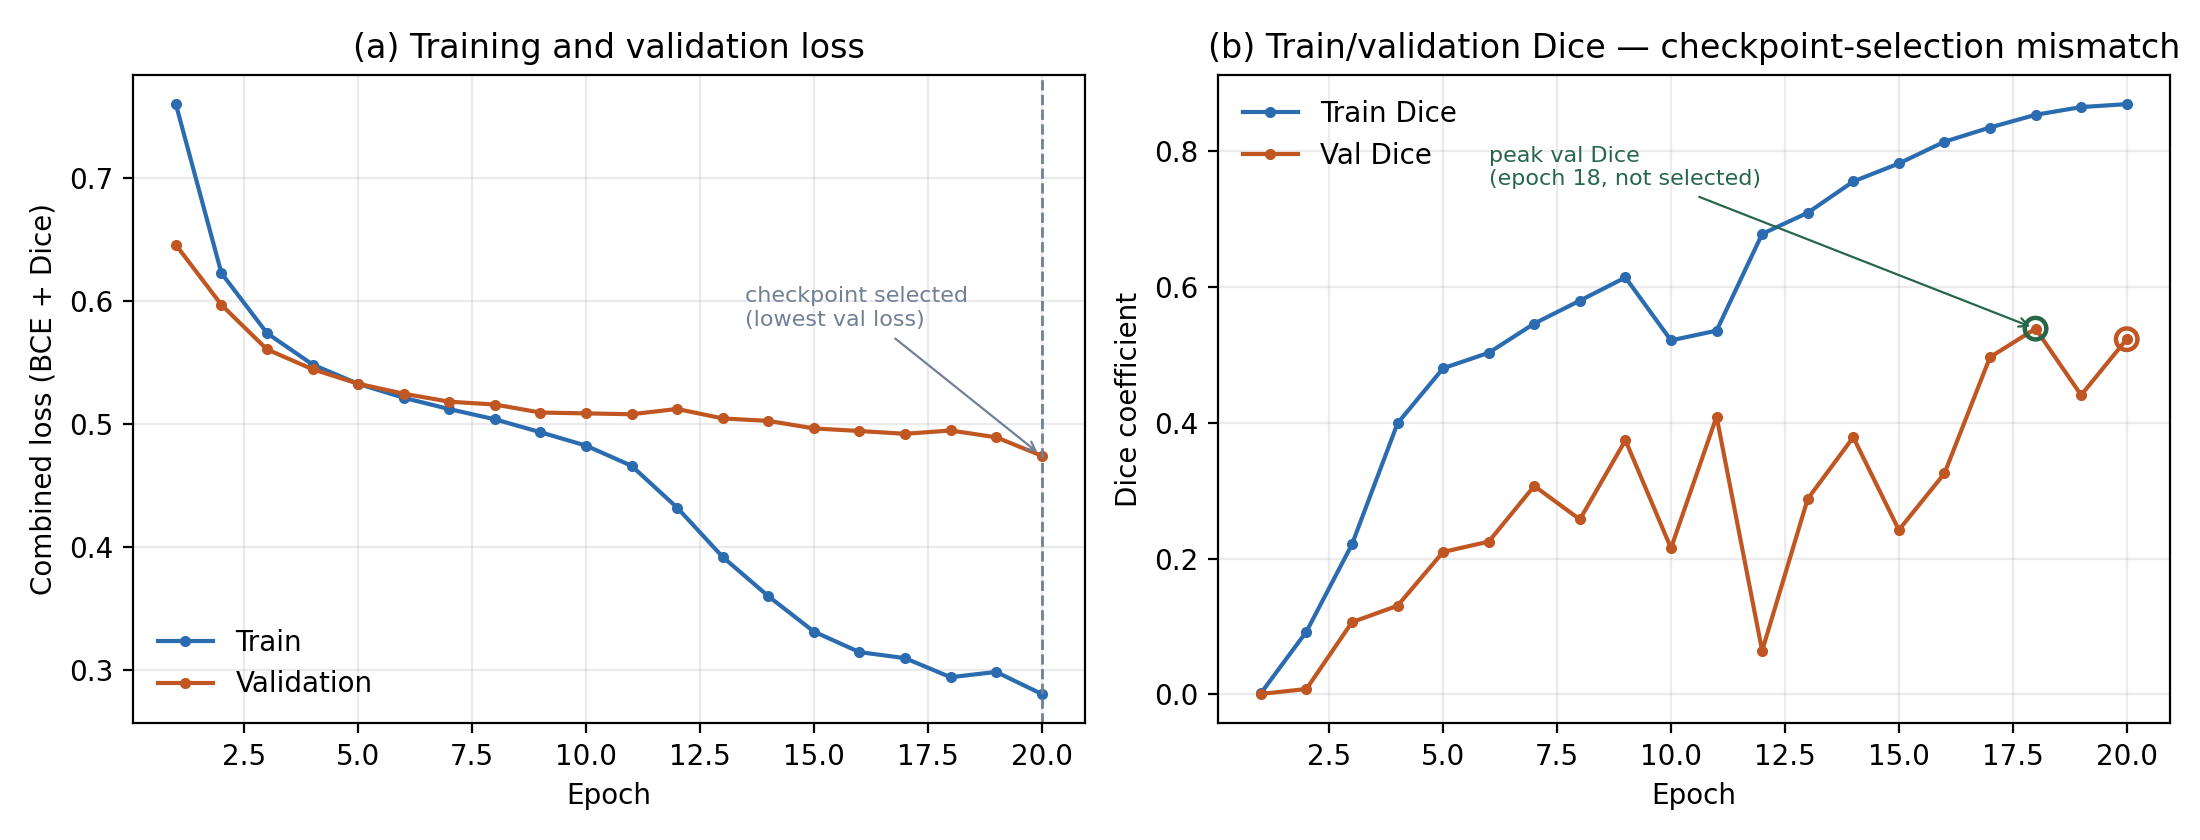
\includegraphics[width=\textwidth]{figures/training_curves.png}
\caption{Training curves for the final run (corrected labels, 20 epochs).
(a) Combined loss decreases smoothly and near-monotonically on both splits;
the checkpoint with the lowest validation loss (epoch 20) is selected as
final. (b) Dice coefficient on the same run: training Dice increases
steadily to 0.87, while validation Dice is markedly noisier and peaks
earlier, at epoch 18 (0.539), one epoch before the checkpoint actually
selected (epoch 20, 0.523).}
\label{fig:training}
\end{figure}

A specific and repeatable methodological finding emerged across all three
runs: the checkpoint selected by lowest validation combined loss is
consistently \emph{not} the checkpoint with the highest validation Dice
score, and the gap between them varies run to run (peak validation Dice
occurred at epoch 10, 15, and 18 in the three respective runs, never at the
final, selected epoch). This is explained by the validation set's small
size --- only 8 positive tiles --- which makes Dice, a metric computed only
over the sparse positive-pixel region, highly sensitive to small changes in
a handful of predictions, whereas the combined loss is dominated by the
binary cross-entropy term, an aggregate over all pixels (99.9975\% of which
are negative) and therefore far smoother epoch to epoch. Checkpoint
selection on validation combined loss, rather than raw Dice, is judged the
more defensible choice specifically because of this instability, though it
is worth noting explicitly that the two criteria do not always agree on
which model is best, and that a model selected this way is not guaranteed
to be the one with maximal segmentation overlap quality on any given run.

Figure~\ref{fig:lossdecomp} isolates the two loss components to make the
mechanism behind this finding directly visible: BCE (Eq.~\ref{eq:bce})
decreases smoothly and almost monotonically from the first epoch --- since
it is an average over $N$ pixels, and the model can lower that average
substantially just by becoming confidently correct on the overwhelming
negative majority, well before it has learned anything useful about the
rare positive class --- while Dice loss (Eq.~\ref{eq:dice}) remains close
to its maximum (worst) value for roughly the first ten epochs before
beginning to improve, since it is computed only from the positive-pixel
overlap and gives the model no credit at all for correct negative
predictions. Since the combined loss (Eq.~\ref{eq:combined}) is an
equal-weighted average of the two, its early- and mid-training trajectory
is effectively governed by BCE alone, which explains why checkpoints
selected by combined loss can diverge from the checkpoint with the best
actual segmentation overlap.

\begin{figure}[htbp]
\centering
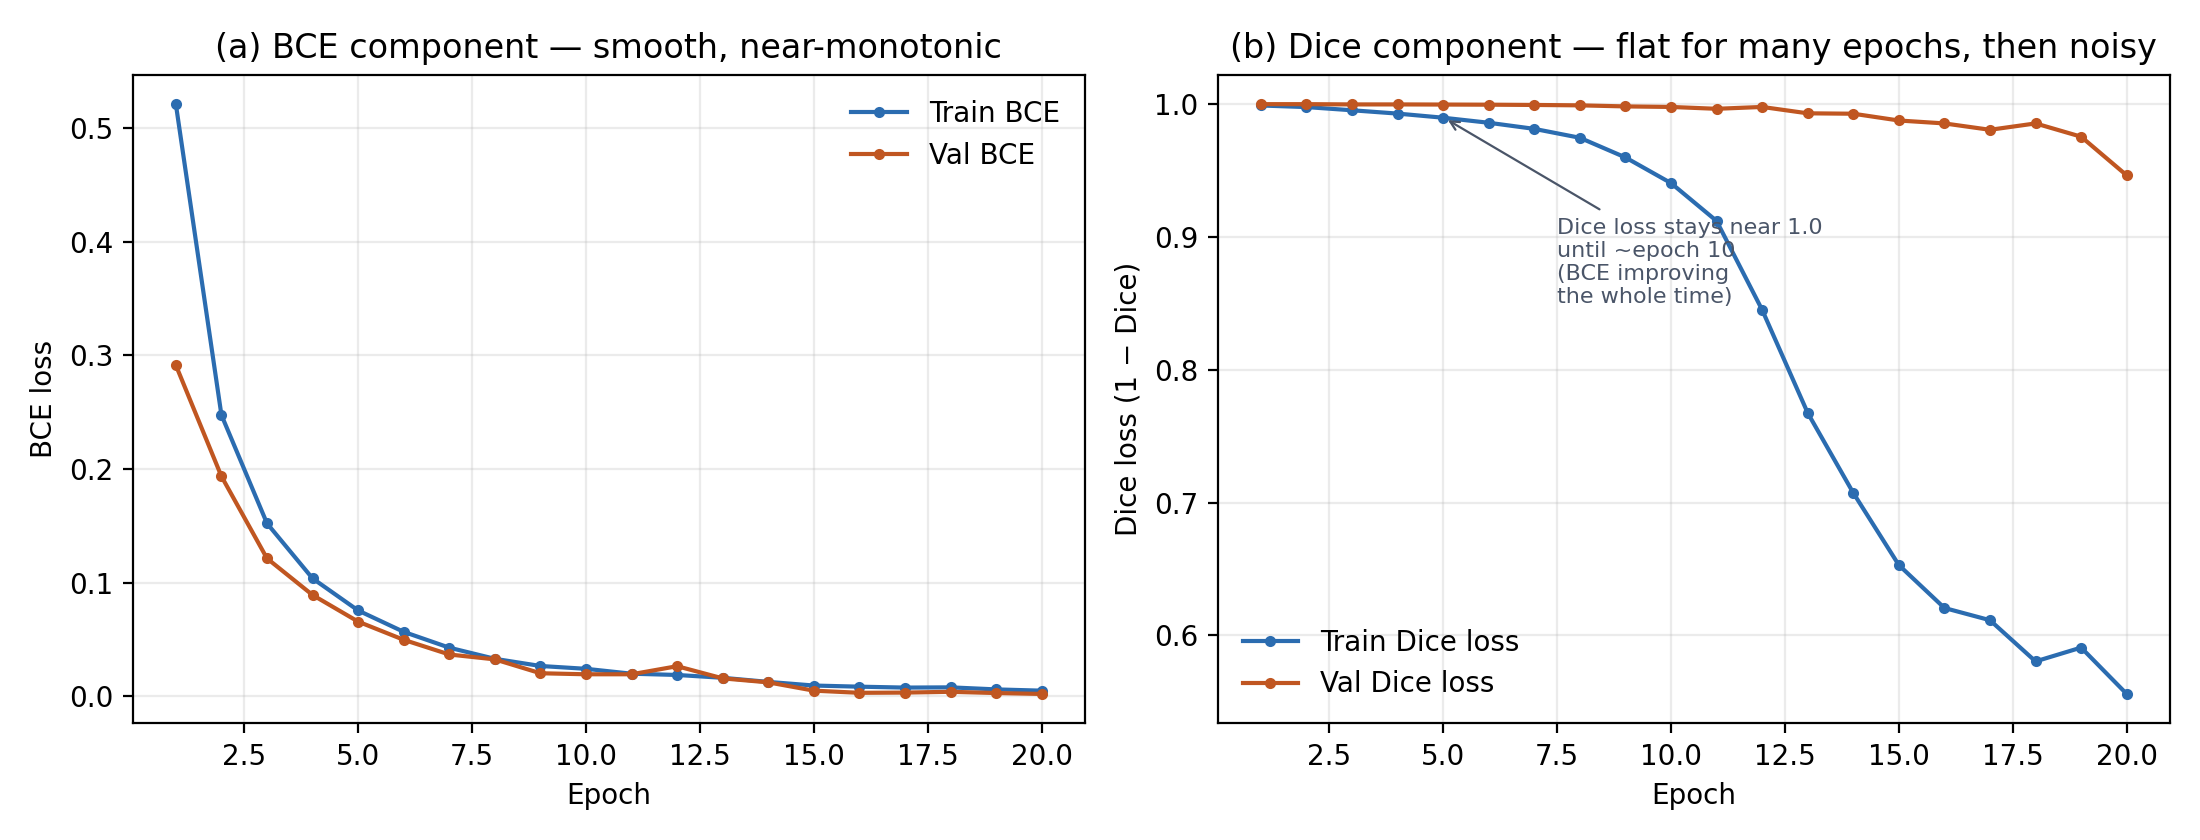
\includegraphics[width=\textwidth]{figures/loss_decomposition.png}
\caption{Decomposition of the combined loss into its BCE and Dice
components (final run, corrected labels). The BCE term drives early
optimization; the Dice term only becomes informative once the model has
already learned to concentrate probability mass on the rare positive
class.}
\label{fig:lossdecomp}
\end{figure}

This checkpoint-selection mismatch was not a one-off observation: it
recurred, in varying degree, across all three full training runs performed
during this project (the first two using pre-audit labels, the third using
the corrected dataset from Section~\ref{sec:audit}), summarized in
Table~\ref{tab:runs}.

\begin{table}[htbp]
\centering
\caption{Comparison across all three full training runs. ``Selected''
refers to the checkpoint chosen by lowest validation combined loss (the
deployed model in each run); ``Peak Dice'' refers to the epoch with the
highest validation Dice score observed anywhere in that run.}
\label{tab:runs}
\begin{tabular}{lccccc}
\toprule
\textbf{Run} & \textbf{Labels} & \textbf{Selected epoch} & \textbf{Selected val Dice} & \textbf{Peak Dice epoch} & \textbf{Peak val Dice} \\
\midrule
Run 1 & pre-audit  & 20 & 0.461 & 10 & 0.556 \\
Run 2 & pre-audit  & 20 & 0.570 & 15 & 0.647 \\
Run 3 & post-audit & 20 & 0.523 & 18 & 0.539 \\
\bottomrule
\end{tabular}
\end{table}

In every run, the selected checkpoint is the final epoch (20), while the
peak-Dice epoch varies unpredictably run to run (10, 15, then 18) --- a
direct consequence of validation Dice being computed over only 8 positive
tiles, and further evidence that raw Dice, on a validation set this small,
should be treated as a noisy diagnostic signal rather than a reliable
epoch-selection criterion. Notably, the gap between the selected and peak
Dice scores narrows substantially in Run 3 (relative gap $\sim$3\%, versus
$\sim$19\% and $\sim$14\% in Runs 1 and 2); this is consistent with, though
not proven to be caused by, the single label correction applied between
Run 2 and Run 3, given the single-run sample size.

\subsection{Full-scene inference and evaluation}
\label{sec:falsepos}
A sliding-window inference pipeline was built to apply the tile-trained
model to full, arbitrarily large scene images: overlapping 640$\times$640
windows are slid across the scene, the model is run on each window
independently, and overlapping predictions are averaged and stitched into
one continuous probability heatmap the size of the original scene.

On the held-out validation scene 20220921\_226\_120 (five known garimpo
sites), every one of the five sites was recovered with maximum predicted
probability (1.00) inside its ground-truth box, and a scan of the entire
scene for probability-0.5 blobs found exactly five, matching the five known
sites with no additional false positives anywhere else in the scene.
Figure~\ref{fig:detection} shows one such example: the predicted heatmap is
visibly faint at the scale of a full 640$\times$640 tile, but a tight crop
around the ground-truth box shows a clear, correctly-located confidence
response, consistent with the quantitative result.

\begin{figure}[htbp]
\centering
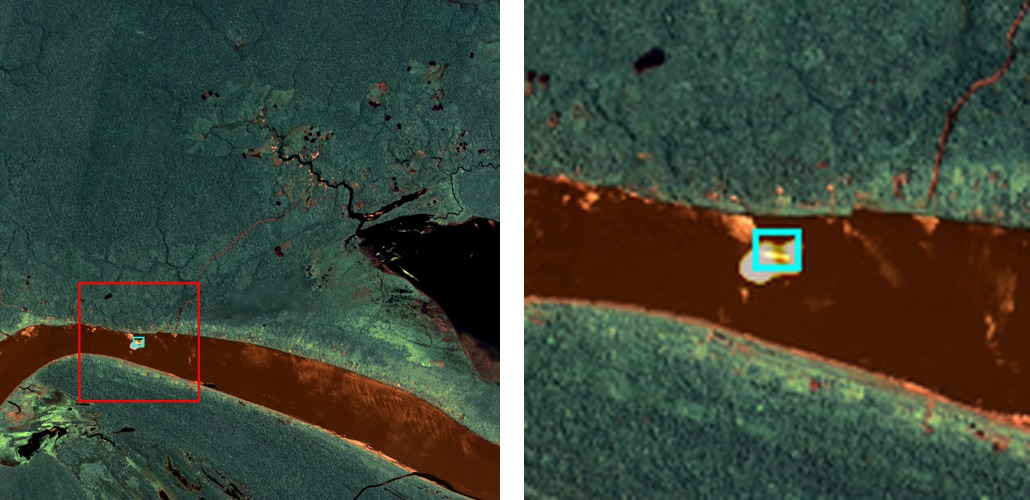
\includegraphics[width=\textwidth]{figures/fig_tile_comparison.jpg}
\caption{Example detection result on a held-out validation tile
(20220921\_226\_120). Left: full tile, with the ground-truth box (cyan) and
the cropped region (red) indicated. Right: 4$\times$ zoom on the crop,
showing the predicted probability heatmap (pale/orange glow) correctly
centered on the ground-truth box.}
\label{fig:detection}
\end{figure}

On the scene with zero labeled positives, 20211015\_226\_121, the same scan
found seven candidate blobs. Four were substantially coincident with
nodata/scene-border pixels, consistent with the artifact sensitivity
documented in Section~\ref{sec:audit}. The remaining three were visually
similar in character to confirmed detections (a bright spot at a small
tributary stream-bend) but sit on data with no ground-truth label at all,
so their status cannot be resolved from the available data alone. A
cross-date check --- scanning the same pixel coordinates across the other
five acquisition dates of the same footprint --- found activation only on
the source date, in every case. This rules out one plausible explanation
(a static, terrain-shape-based shortcut, which would be expected to fire
identically on every date of the same, unchanged terrain) but does not
confirm the alternative (a genuine, undocumented mining site); it is
reported here as an open, unresolved finding rather than a settled one.

Figure~\ref{fig:fullscene} shows the full stitched heatmap for the
validation scene discussed above, alongside a zoomed inset on its main
detection cluster (four of the six known boxes in this scene sit within
approximately 150 px of one another, near a tiling-grid corner). The
zoomed view also makes visible, incidentally, the duplicate-labeling
artifact identified in Section~\ref{sec:audit}: overlapping ground-truth
box outlines at a shared tile boundary, corresponding to the same physical
site independently boxed in two adjacent tiles before the box-merging
correction described there.

\begin{figure}[htbp]
\centering
\begin{subfigure}[b]{0.48\textwidth}
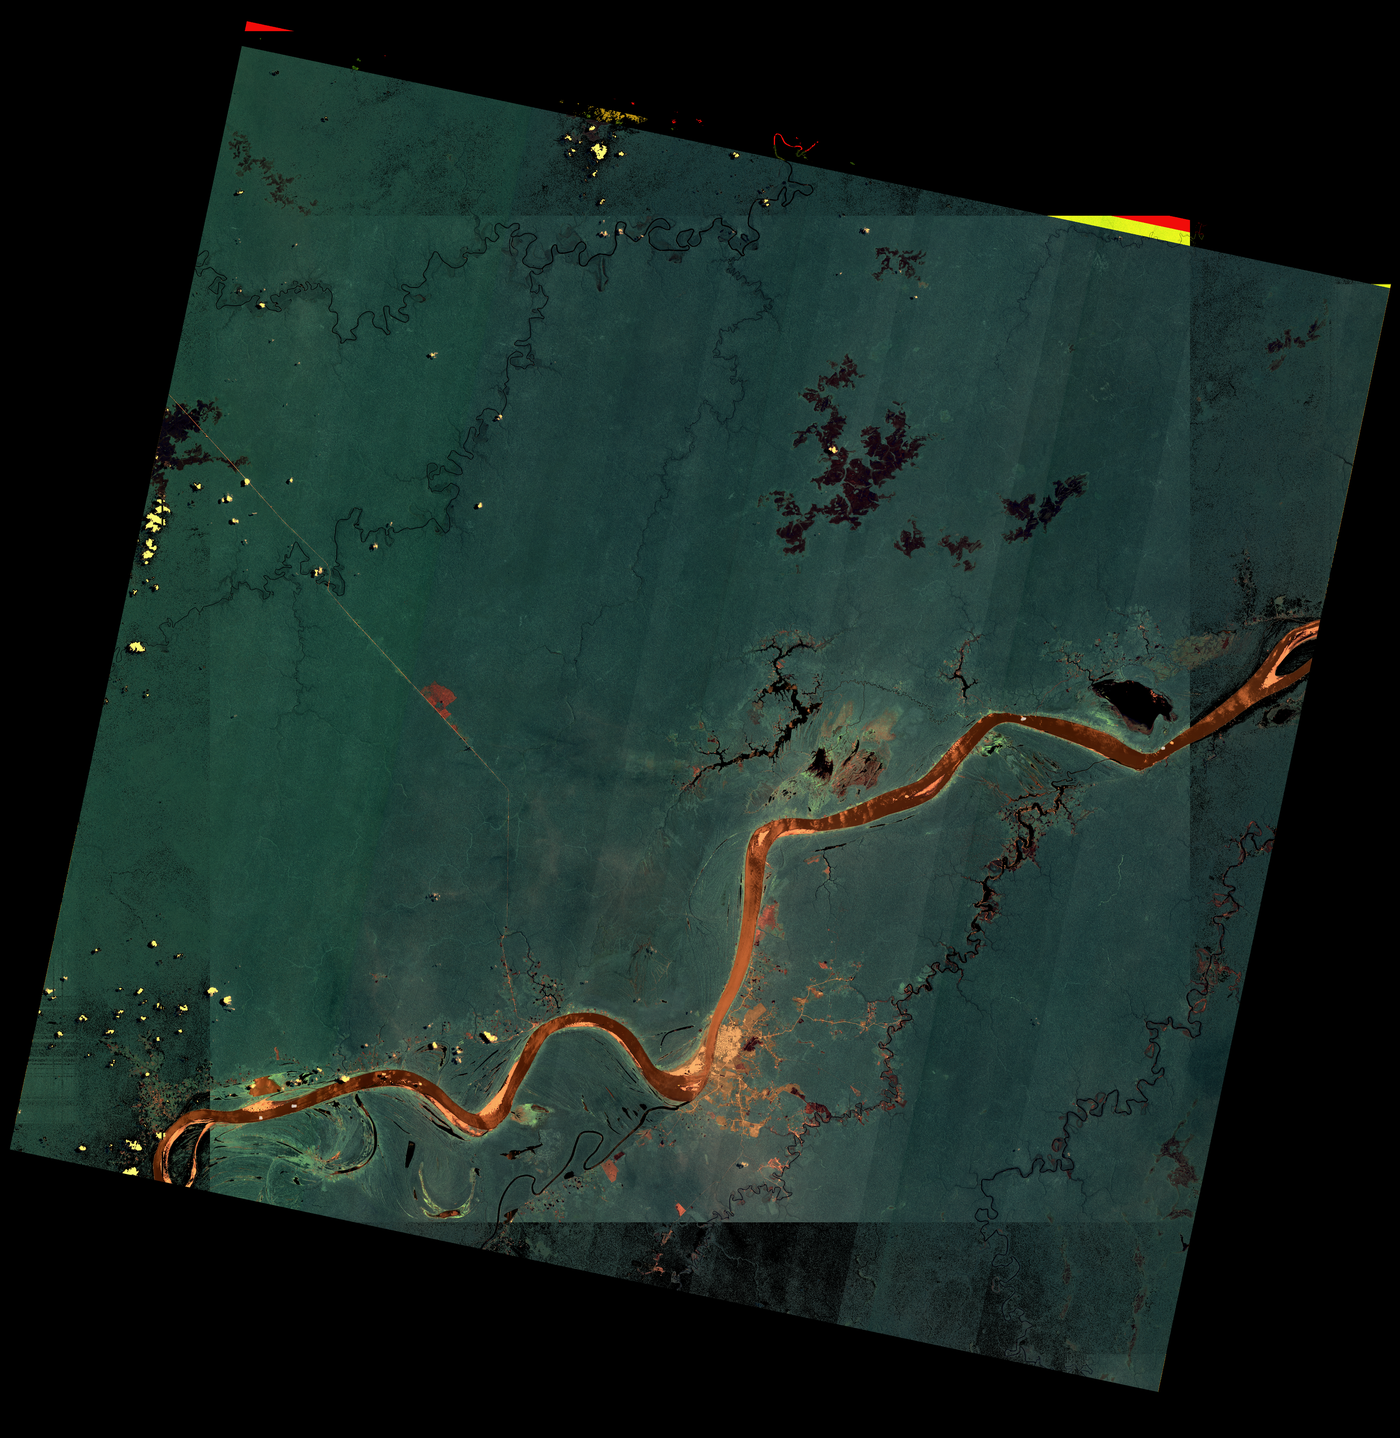
\includegraphics[width=\textwidth]{figures/fig_fullscene_overview.png}
\caption{Full stitched probability heatmap over the entire scene.}
\end{subfigure}
\hfill
\begin{subfigure}[b]{0.48\textwidth}
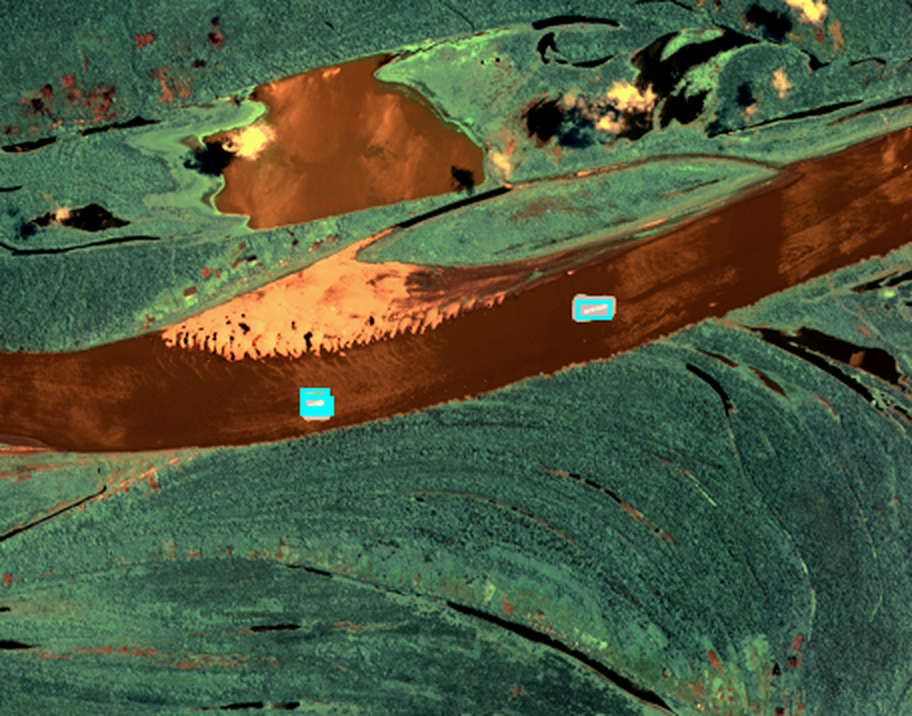
\includegraphics[width=\textwidth]{figures/fig_fullscene_inset.png}
\caption{Zoomed inset on the main detection cluster, with ground-truth
box outlines (cyan) overlaid.}
\end{subfigure}
\caption{Full-scene sliding-window inference result, validation scene
20220921\_226\_120. The isolated colored strip near the top edge of (a) is
a data-quality flag baked into the source imagery itself (confirmed by
direct pixel inspection, not a model prediction).}
\label{fig:fullscene}
\end{figure}

Applying the same evaluation across all 13 available scenes, and after
correcting for a small number of duplicate labels (adjacent tiles sharing a
grid boundary independently boxing the same physical site, merged via
literal-overlap detection: 42 raw boxes reduced to 34 unique sites), yields
the precision/recall summary in Table~\ref{tab:evalsummary} and
Figure~\ref{fig:byscene}.

\begin{table}[htbp]
\centering
\caption{Detection performance across all 13 scenes, threshold = 0.5.}
\label{tab:evalsummary}
\begin{tabular}{lrrrrr}
\toprule
\textbf{Split} & \textbf{TP} & \textbf{FP} & \textbf{FN} & \textbf{Precision} & \textbf{Recall} \\
\midrule
All 13 scenes    & 34 & 78 & 0 & 0.304 & 1.000 \\
Training scenes  & 28 & 66 & 0 & 0.298 & 1.000 \\
Validation scenes & 6 & 12 & 0 & 0.333 & 1.000 \\
\bottomrule
\end{tabular}
\end{table}

\begin{figure}[htbp]
\centering
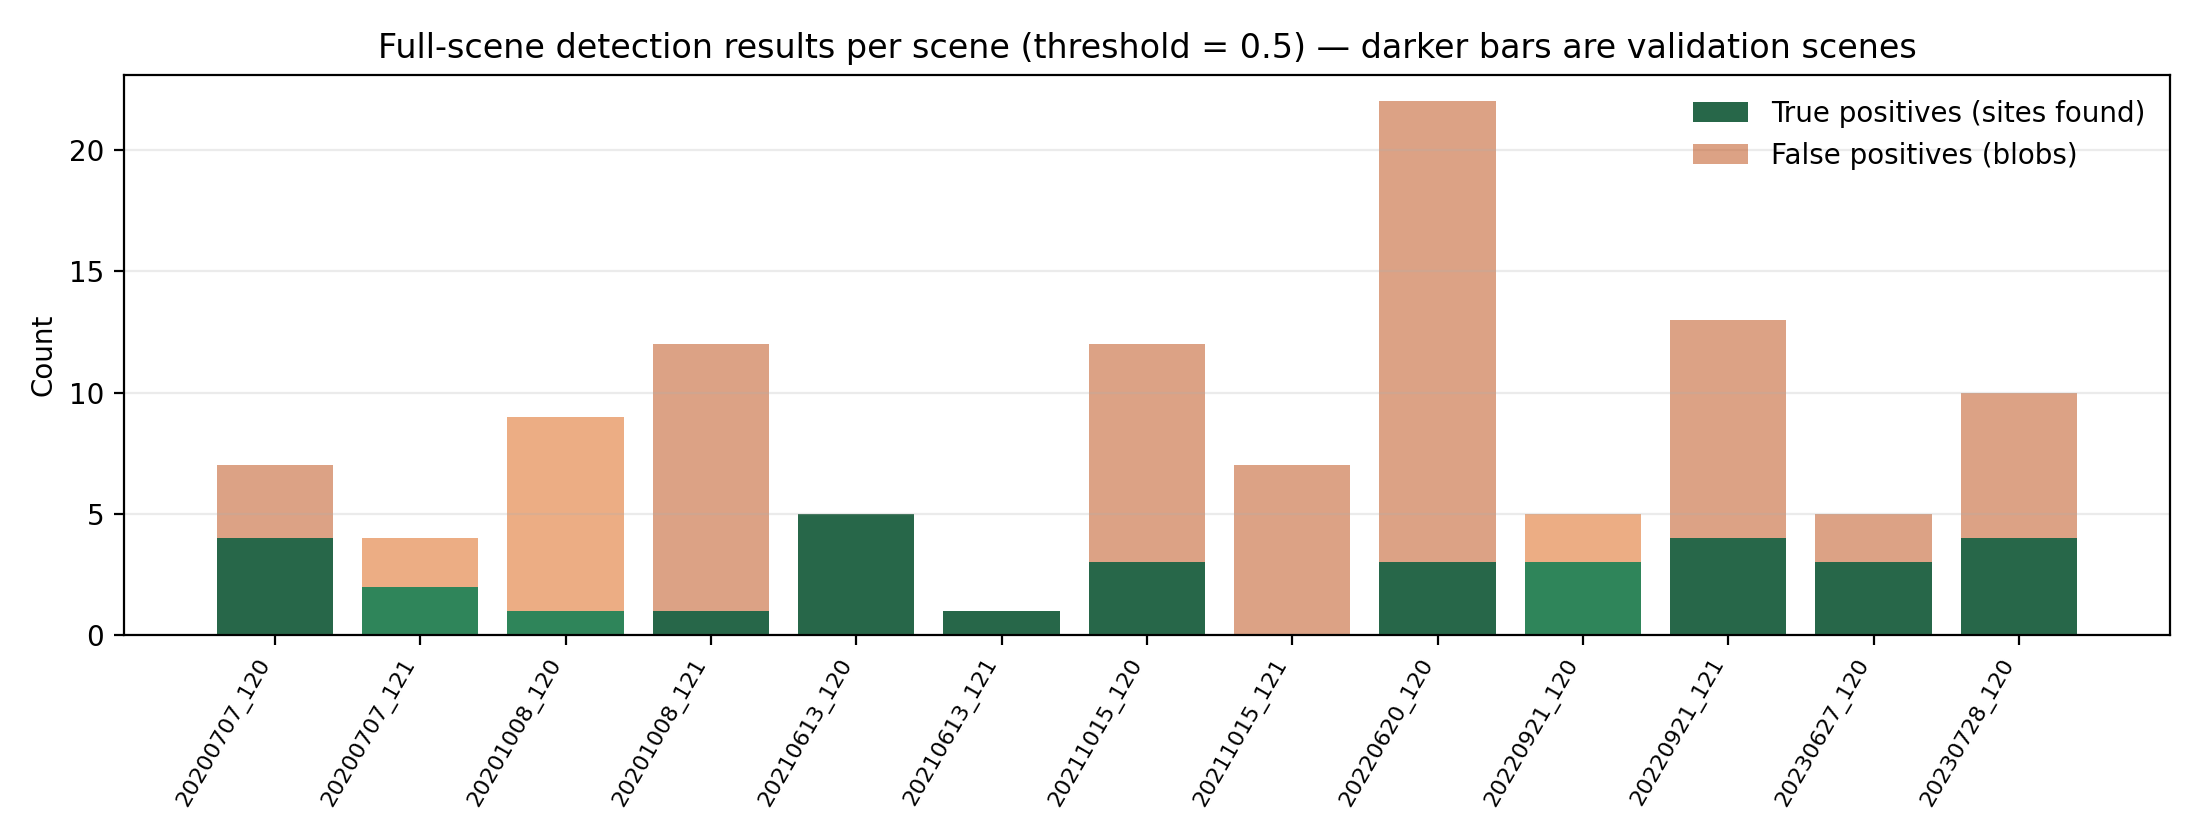
\includegraphics[width=\textwidth]{figures/detection_by_scene.png}
\caption{True and false positives per scene at threshold 0.5. Darker bars
indicate validation-split scenes. The single largest source of false
positives, scene 20220620\_226\_120 (19 of 22 detections false), is an
outlier not yet explained and flagged for follow-up.}
\label{fig:byscene}
\end{figure}

Recall is exactly 100\% across every split, a result confirmed to follow
directly from the earlier per-tile checks (every known site had already been
independently confirmed to overlap a detected blob before scene-level
merging), rather than an artifact of a lenient matching threshold. Of the 78
total false positives, 34 coincide with the documented nodata/artifact
sensitivity; excluding these gives an adjusted precision of 43.6\% on
otherwise clean imagery. Table~\ref{tab:fpbreakdown} gives the full
per-scene breakdown, computed directly within the same matching pass as
the TP/FP counts themselves (not derived by combining separate analysis
runs), confirming the nodata/clean split exactly ($34 + 44 = 78$).

\begin{table}[htbp]
\centering
\caption{False-positive breakdown by scene and cause, threshold = 0.5.}
\label{tab:fpbreakdown}
\begin{tabular}{lccccc}
\toprule
\textbf{Scene} & \textbf{Split} & \textbf{TP} & \textbf{FP} & \textbf{FP (nodata)} & \textbf{FP (clean)} \\
\midrule
20200707\_226\_120 & train & 4 & 3  & 0 & 3 \\
20200707\_226\_121 & val   & 2 & 2  & 1 & 1 \\
20201008\_226\_120 & val   & 1 & 8  & 5 & 3 \\
20201008\_226\_121 & train & 1 & 11 & 7 & 4 \\
20210613\_226\_120 & train & 5 & 0  & 0 & 0 \\
20210613\_226\_121 & train & 1 & 0  & 0 & 0 \\
20211015\_226\_120 & train & 3 & 9  & 4 & 5 \\
20211015\_226\_121 & train & 0 & 7  & 3 & 4 \\
20220620\_226\_120 & train & 3 & 19 & 7 & 12 \\
20220921\_226\_120 & val   & 3 & 2  & 0 & 2 \\
20220921\_226\_121 & train & 4 & 9  & 7 & 2 \\
20230627\_226\_120 & train & 3 & 2  & 0 & 2 \\
20230728\_226\_120 & train & 4 & 6  & 0 & 6 \\
\bottomrule
\end{tabular}
\end{table}

Two scenes stand out on inspection. The 20220620\_226\_120 outlier flagged
above is confirmed to be dominated by clean (non-nodata) false positives
(12 of 19), meaning its high false-positive count is not simply an
extension of the already-understood artifact issue and remains an open
item. Conversely, 20201008\_226\_121 and 20220921\_226\_121 both show
nodata false positives outweighing clean ones (7 of 11 and 7 of 9,
respectively), consistent with the documented sensitivity and not, on
their own, cause for additional concern.

A closer investigation of the ``clean'' (non-nodata) false positives was
prompted by an observation made during an early map-interface prototyping
exercise: several detections appeared, at first glance, to
sit well inland with no visible water nearby, raising the concern that the
model might be responding to bare or cleared land in general rather than
any water-related signature. This was investigated in two stages, and the
first was explicitly discarded once shown to be flawed: an initial proximity
check --- distance from each false positive to the nearest water pixel,
using a color-based river mask built directly from the imagery and
validated visually against the true river channel and its tributaries ---
showed roughly 41\% of the 78 false positives falling within a loose 200 px
buffer of water. This number is not diagnostic on its own, however: the
same check applied to the 34 true positives shows them at 100\% within a
much tighter 30 px buffer (median distance 0 px) --- essentially every
detection, correct or not, falls somewhere near the river, simply because
that is where both real mining activity and the model's attention
concentrate. Raw proximity cannot separate a genuine water-related
confusion from ordinary river-corridor geography.

A stricter, spectral test resolves this: rather than asking whether a false
positive is merely \emph{near} water, it asks whether the false positive's
own pixels fall \emph{inside} the calibrated water/sediment color
signature. This reclassifies the false positives into mutually exclusive,
fully reconciled categories, summarized in
Table~\ref{tab:fpcauses}. Of the 44 clean false positives, 18 (23.1\% of
all 78) sit directly on water- or sediment-colored pixels --- consistent
with bare sediment and mining tailings sharing the same warm, low-saturation
tone as exposed riverbank sediment in this sensor's true-color rendering,
a plausible and specific causal mechanism rather than mere proximity. A
further 10 (12.8\%) sit adjacent to a nodata/seam region that falls just
outside the detection's own bounding box (missed by the tighter check in
Section~\ref{sec:audit}, which only examined the box interior), and 4
(5.1\%) sit beside an interior, non-border-touching dark patch consistent
with cloud shadow --- a previously undocumented false-positive mechanism.
The remaining 12 (15.4\%) have no confident explanation under any of these
checks and are reported as genuinely unresolved, rather than forced into
one of the other categories. Manual review of the single highest-confidence
unresolved case found it sitting at a tight bend of a narrow, dark tributary
creek --- plausibly still water-related, but with a color signature (dark,
low-saturation) that falls outside the range calibrated on the wide,
sediment-tinted main channel; the water mask's known under-sensitivity to
narrow, shaded tributaries makes the true unresolved count more likely an
upper bound than a precise estimate of a distinct failure mode.

\begin{table}[htbp]
\centering
\caption{Root-cause breakdown of all 78 false positives, threshold = 0.5.
Categories are mutually exclusive and reconcile exactly to the total.}
\label{tab:fpcauses}
\begin{tabular}{lrr}
\toprule
\textbf{Cause} & \textbf{Count} & \textbf{\% of 78} \\
\midrule
Nodata/seam within own bounding box (Section~\ref{sec:audit}) & 34 & 43.6\% \\
Water/sediment-colored pixels & 18 & 23.1\% \\
Nodata/seam just outside bounding box & 10 & 12.8\% \\
Interior cloud shadow & 4 & 5.1\% \\
Unexplained & 12 & 15.4\% \\
\bottomrule
\end{tabular}
\end{table}

Taken together, 84.6\% of all false positives (66 of 78) now have a
specific, visually-confirmed or spectrally-verified explanation, spanning
three related but distinct mechanisms --- scan/mosaic artifacts, genuine
spectral similarity between mining-related sediment and natural riverbank
sediment, and cloud shadow --- none of which point to the model responding
to arbitrary or unrelated terrain.

\subsubsection{Geomorphological interpretation}
\label{sec:geomorph}
The dominant false-positive mechanism identified above --- spectral
confusion with natural water/sediment features --- is not an arbitrary
model weakness; it follows directly from the fluvial geomorphology of the
study reach, and connects this project's results back to the founding
observation of Monteiro (2024).

Madeira River gold is secondary (alluvial) gold, eroded from Andean source
rocks and transported downstream as bedload and suspended sediment
(Table~\ref{tab:river}). In a meandering, anabranching channel, flow
velocity drops sharply on the inside of a bend, and it is precisely there
--- on the resulting \emph{point bar} --- that this sediment, including
its denser gold fraction, preferentially settles. This is a well-established
physical sorting process, not a mining-specific phenomenon.
Figure~\ref{fig:geomorph} illustrates the mechanism.

\begin{figure}[htbp]
\centering
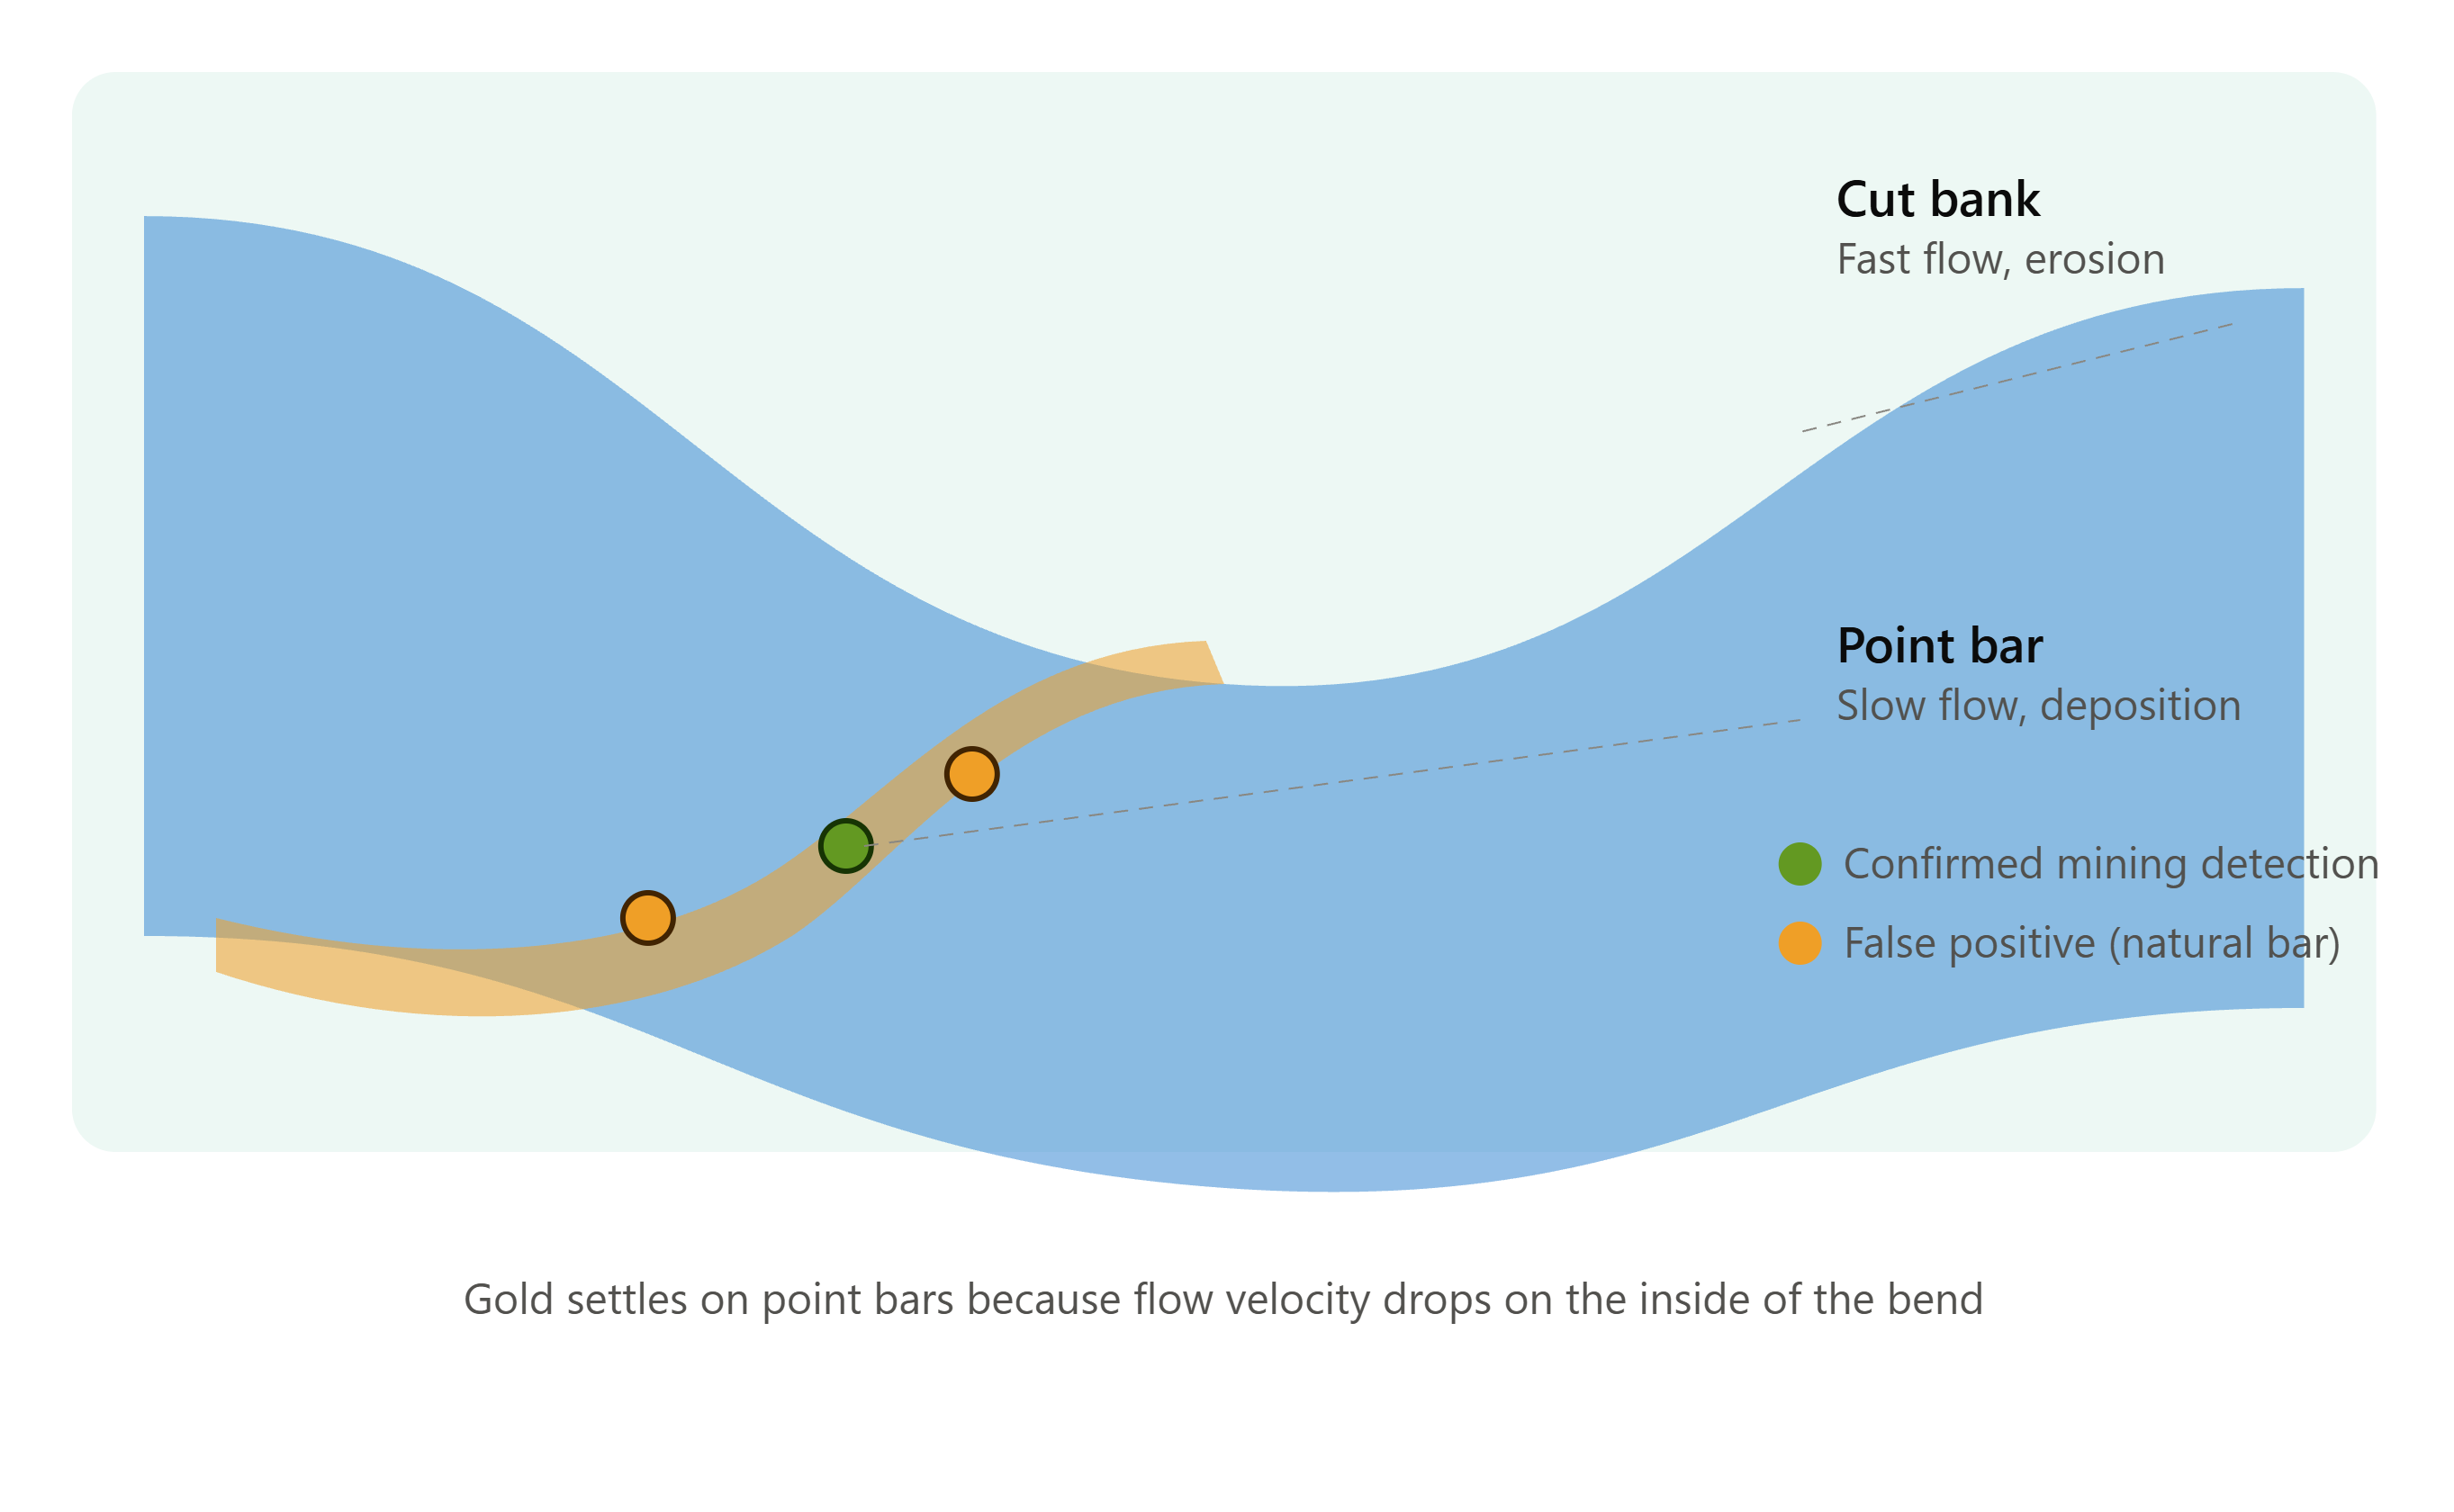
\includegraphics[width=0.85\textwidth]{figures/fig_geomorph.png}
\caption{Schematic river meander. Flow slows on the inside of the bend,
depositing sediment (the point bar, orange) --- including its alluvial
gold fraction --- while the outer bank (cut bank) erodes under faster
flow. Both real mining detections and the model's dominant false-positive
mechanism cluster on the point bar, since actively-mined and naturally
undisturbed sediment share a similar true-color spectral signature.}
\label{fig:geomorph}
\end{figure}

This single mechanism explains three separate observations at once.
First, it explains why Monteiro (2024) found manually-digitized barge
locations correlating with fluvial bars: miners target point bars because
that is physically where the gold concentrates, not by coincidence.
Second, it explains why this project's true positives sit essentially on
the water/sediment mask (median distance 0 px, Section~\ref{sec:falsepos}):
the model has correctly learned to associate garimpo with this
depositional signature. Third, and most usefully, it explains the model's
principal failure mode: an actively-mined point bar and an entirely
undisturbed one are composed of the same pale, low-vegetation sediment,
and are often close to spectrally indistinguishable in true-color RGB
imagery alone. The model has therefore learned a genuine and geologically
correct cue --- sediment deposition zones --- without yet being able to
separate \emph{active} disturbance from a merely \emph{favorable} location.
This directly motivates the near-infrared reintroduction proposed in
Section~\ref{sec:nextsteps}: disturbed, freshly-worked sediment differs
from an undisturbed bar in moisture content and grain sorting in ways
that are known to be more separable in the near-infrared than in visible
light, offering a physically-grounded route to reducing this specific
failure mode rather than a purely data-driven one.

Separately, a visually striking example encountered during interface
development --- a high-confidence marker appearing to sit on an unrelated
inland forest clearing, well away from any labeled site --- was traced to
a different cause entirely: the scene in question is not one of the two
dates for which exact footprint coordinates are available, and inherits
the approximate-georeferencing limitation of the prototype map interface
(Section~\ref{sec:nextsteps}): the current implementation reuses one
date's footprint coordinates for all other dates of the same path/row, a
reasonable approximation given CBERS's documented $\pm$5 km track
stability but not pixel-exact across dates (a marker \emph{display}
position offset, not a detection or model issue). Verification on an
actual reference-date scene
confirmed the underlying pixel-to-coordinate transform itself is correct,
with only a small residual offset attributable to approximating the true
rotated scene footprint with a north-aligned rectangle.

At this operating point, the
detector's error profile --- never missing a known site, at the cost of a
meaningful false-positive rate, now attributable in large part to specific
and plausible visual/spectral confusions rather than arbitrary noise --- is
a reasonable fit for a first-pass screening tool, where a missed site is a
materially worse outcome than an extra location flagged for human review,
though the validation-split numbers in Table~\ref{tab:evalsummary} are
based on only three scenes and should not be over-interpreted as a tightly
estimated figure.

\section{Next Steps}
\label{sec:nextsteps}

\begin{enumerate}[nosep]
  \item Build and validate an interactive map interface displaying
        detections on a real satellite basemap, using footprint
        coordinates recovered from CBERS product metadata, with
        confidence-coded detection markers --- architecture prototyped but
        not yet included as validated project output.
  \item Recover precise, per-date georeferencing (rather than the current
        one-date-per-footprint approximation) using the recovered raw band
        GeoTIFFs, and reintroduce the near-infrared band into the training
        pipeline.
  \item Investigate the false-positive outlier at scene
        20220620\_226\_120 (19 of 22 detections false, well above any other
        scene).
  \item Reduce the model's residual sensitivity to nodata/mosaic-seam
        artifacts, either by masking such regions at inference time or by
        targeted hard-negative training on artifact-adjacent tiles.
  \item Investigate whether the near-infrared band (recoverable from the
        raw band GeoTIFFs, per the item above) can help the model
        separate genuine turbid-water/mining-plume signatures from the
        spectrally similar natural sediment identified as the largest
        single explained cause of false positives (Table~\ref{tab:fpcauses}),
        since RGB true-color imagery alone does not appear sufficient to
        reliably distinguish them. A river-proximity post-filter was
        considered and explicitly ruled out as a fix: true positives sit
        just as consistently near water as false positives do (both
        approach 100\% within a loose buffer), so proximity alone cannot
        discriminate between them --- the spectral similarity itself, not
        mere location, is the mechanism to address.
  \item Investigate the 12 false positives that remain unexplained after
        the nodata/seam, spectral, and cloud-shadow checks
        (Section~\ref{sec:falsepos}) --- most likely by extending the
        water/sediment color mask to better cover narrow, shadowed
        tributary streams, which the current mask under-detects.
  \item Build a coordinate-based, on-demand interface: given a
        user-selected location and time on the map, run inference directly
        on that location rather than requiring a full pre-computed
        scene-level heatmap.
  \item Address the observed train/validation performance gap (final-epoch
        train Dice 0.87 vs.\ validation Dice 0.52), through stronger
        regularization, more aggressive augmentation, or additional labeled
        data.
  \item Given the two-footprint geographic limitation identified in
        Section~\ref{sec:model}, evaluate whether a cross-validation scheme
        (rotating which scenes are held out) would give a more statistically
        robust performance estimate than the current single fixed split.
  \item Extend the false-positive analysis with a precision--recall curve
        across multiple probability thresholds, to characterize the
        precision/recall trade-off beyond the single operating point
        reported here.
  \item Compare model detections against the manually-digitized locations
        reported by Monteiro (2024), where acquisition dates overlap, as an
        external validation reference.
\end{enumerate}

\section*{Acknowledgements}
This work is conducted under a research internship agreement between EMINES
School of Industrial Management (UM6P) and the Departamento de
Geoci\^encias (DEGEO), Universidade Federal do Amazonas (UFAM). We thank
Anna Beatriz de Oliveira Monteiro and Prof.\ Naziano Pantoja Filizola
J\'unior for the foundational thesis work this project builds upon.

\section*{References}
\begin{footnotesize}
\noindent
Monteiro, A.\ B.\ O.\ (2024). Identifica\c{c}\~ao e an\'alise do garimpo de
ouro no rio Madeira atrav\'es do uso de imagens de radar e \'opticas
relacionado aos aspectos hidrodin\^amicos, geomorfol\'ogicos e geol\'ogicos.
Trabalho Final de Gradua\c{c}\~ao (Bacharelado em Geologia), Universidade
Federal do Amazonas, Manaus.

\noindent
Bastos, W.\ R.; Lacerda, L.\ D.\ (2004). A contamina\c{c}\~ao por merc\'urio
na bacia do rio Madeira: uma breve revis\~ao. Geochimica Brasiliensis,
18(2).

\noindent
INPE -- Instituto Nacional de Pesquisas Espaciais (2019). C\^ameras
Imageadoras CBERS 04A. Available at:
\url{http://www.cbers.inpe.br/sobre/cameras/cbers04a.php}.
\end{footnotesize}

\end{document}